
En esta sección se presentan los resultados preliminares del proceso de modelamiento para la estimación del Índice de Pobreza Multidimensional (IPM) 2024 mediante un enfoque de estimación para áreas pequeñas. El ejercicio desarrollado tuvo como propósito construir y evaluar una primera aproximación metodológica que permitiera combinar la estimación directa del IPM a nivel departamental, proveniente de la Encuesta Nacional de Calidad de Vida (ECV) 2024, con un conjunto de covariables auxiliares disponibles a nivel municipal.

El proceso analítico se estructuró en cuatro momentos principales:
\begin{enumerate}
    \item Se construyó una base analítica departamental a partir de la agregación de covariables municipales.
    \item Se ajustaron distintos modelos lineales exploratorios con diferentes combinaciones de variables.
    \item Se estimaron dos variantes del modelo Fay–Herriot.
    \item Se aplicaron los coeficientes obtenidos para generar una predicción sintética municipal del IPM 2024, acompañada de ejercicios preliminares de validación y diagnóstico espacial.
\end{enumerate}

\section{Insumos utilizados}
La base de modelamiento estuvo conformada por la estimación directa del IPM 2024 a nivel departamental, su varianza directa asociada y un conjunto de covariables auxiliares agregadas desde el nivel municipal. La varianza directa se calculó como el cuadrado del error estándar reportado para cada estimación directa:
\begin{equation}
v_d = [SE(\hat{y}_d)]^2
\end{equation}

Donde:
\begin{itemize}
    \item $\hat{y}_d$: IPM directo estimado para el departamento $d$.
    \item $SE(\hat{y}_d)$: error estándar de la estimación directa.
    \item $v_d$: varianza directa asociada al departamento $d$.
\end{itemize}

Las covariables auxiliares incluidas corresponden a tres bloques conceptuales relacionados con las dimensiones del IPM: salud, educación e infraestructura básica. Entre las variables consideradas se encuentran indicadores de aseguramiento en salud, mortalidad infantil, repitencia, cobertura educativa, deserción, reprobación, cobertura de acueducto, cobertura de alcantarillado, cobertura de aseo e infraestructura básica.

\section{Modelos exploratorios OLS}
Antes de ajustar el modelo Fay–Herriot, se estimaron distintos modelos lineales ordinarios con fines exploratorios. Estos modelos no se asumieron como estimadores finales del IPM, sino como una etapa de apoyo para revisar la dirección de las relaciones entre variables, la estabilidad de los coeficientes y la pertinencia de diferentes grupos de covariables.

La forma general de estos modelos fue:
\begin{equation}
IPM_d = \beta_0 + \beta_1 X_{1d} + \beta_2 X_{2d} + \dots + \beta_k X_{kd} + \varepsilon_d
\end{equation}

Donde:
\begin{itemize}
    \item $IPM_d$: IPM directo del departamento $d$.
    \item $\beta_0$: intercepto del modelo.
    \item $\beta_1, \beta_2, \dots, \beta_k$: coeficientes asociados a cada covariable.
    \item $X_{1d}, X_{2d}, \dots, X_{kd}$: covariables auxiliares agregadas para el departamento $d$.
    \item $\varepsilon_d$: término de error del modelo.
\end{itemize}

La comparación entre especificaciones se realizó mediante $R^2$, $R^2$ ajustado, AIC, BIC, RMSE, MAE y revisión de multicolinealidad mediante el factor de inflación de la varianza (VIF). Esta etapa permitió identificar modelos con buen desempeño estadístico, pero también priorizar especificaciones parsimoniosas y conceptualmente consistentes con las dimensiones del IPM.

\begin{figure}[H]
    \centering
    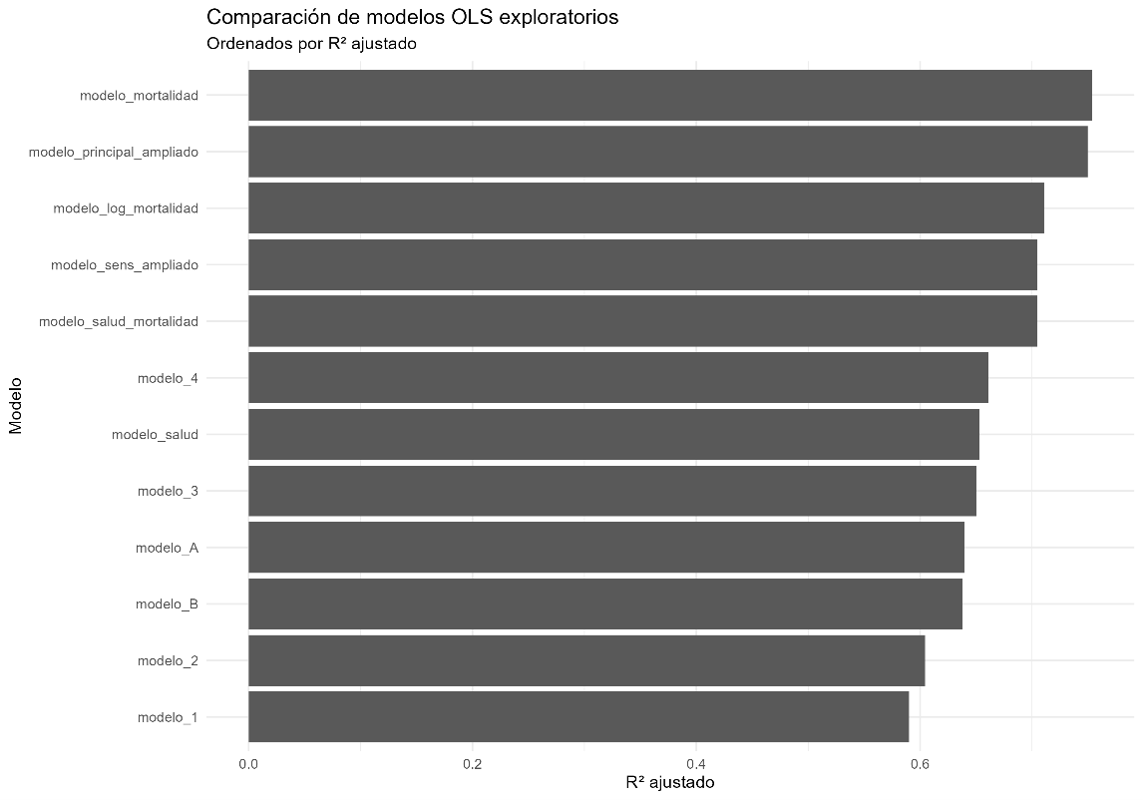
\includegraphics[width=0.65\textwidth]{fig/figures/Comparacion_OLS_exploratorios.png}
    \caption{}
\end{figure}
    \textbf{Fuente:} elaboración propia con base en estimaciones del script de modelamiento.
    
\begin{figure}[H]
    \centering
    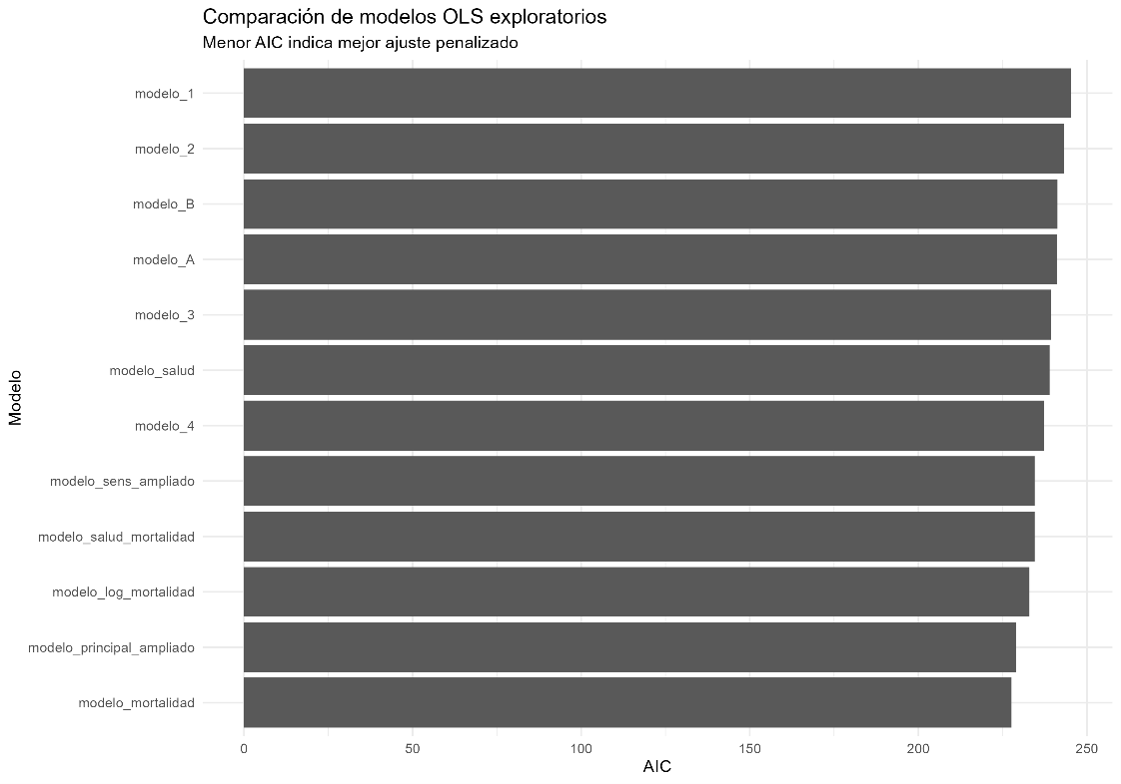
\includegraphics[width=0.65\textwidth]{fig/figures/Comparacion_OLS_exploratorios_2.png}
    \caption{}
    \textbf{Fuente:} elaboración propia con base en estimaciones del script de modelamiento.
\end{figure}

A partir de esta revisión exploratoria se seleccionaron dos especificaciones candidatas para el modelo Fay–Herriot: el modelo principal (que incluyó repitencia, infraestructura básica y mortalidad infantil) y el modelo de sensibilidad (que reemplazó la mortalidad infantil por su transformación logarítmica).

\section{Formulación del modelo Fay–Herriot}
El modelo Fay–Herriot utilizado se expresa de la siguiente manera:

\begin{equation}
    \hat{y}_d = x'_d \beta + u_d + e_d
\end{equation}

Donde $\hat{y}_d$ es la estimación directa del IPM para el departamento $d$, $x'_d$ es el vector de covariables auxiliares, $\beta$ es el vector de coeficientes, $u_d$ es el efecto aleatorio del área y $e_d$ es el error muestral asociado. Los componentes aleatorios se definen así:

\begin{align}
    u_d &\sim N(0, \sigma^2_u) \\
    e_d &\sim N(0, v_d)
\end{align}

El modelo principal se formuló como:

\begin{equation}
    \begin{split}
        IPM_d = \beta_0 + \beta_1(\text{repitencia}_d) + \beta_2(\text{infraestructura básica}_d) + \\
        \beta_3(\text{mortalidad infantil}_d) + u_d + e_d
    \end{split}
\end{equation}

El modelo de sensibilidad se formuló como:
\begin{equation}
    \begin{split}
        IPM_d = \beta_0 + \beta_1(\text{repitencia}_d) + \beta_2(\text{infraestructura básica}_d) + \\
        \beta_3[\log(1 + \text{mortalidad infantil}_d)] + u_d + e_d
    \end{split}
\end{equation}

Ambos modelos fueron ajustados mediante REML utilizando la función Fay–Herriot en R.

\section{Resultados del modelo Fay–Herriot}
Los dos modelos Fay–Herriot convergieron correctamente. No obstante, el modelo principal presentó mejores criterios de ajuste que el modelo de sensibilidad. El modelo principal obtuvo un AIC de 227,26 y un BIC de 234,75, mientras que el modelo de sensibilidad obtuvo un AIC de 232,84 y un BIC de 240,32. Por tanto, el modelo principal se adoptó como especificación de referencia para la interpretación preliminar de resultados.

En el modelo principal, los coeficientes estimados fueron consistentes con la interpretación esperada. La repitencia presentó un coeficiente positivo de 393,71, lo que indica que mayores niveles de repitencia se asocian con mayores niveles de pobreza multidimensional. La infraestructura básica presentó un coeficiente negativo de -18,48, lo que sugiere que mejores coberturas de acueducto, alcantarillado y aseo se asocian con menores niveles de IPM. La mortalidad infantil también presentó una relación positiva con el IPM, con un coeficiente de 0,12, lo cual es coherente con su interpretación como proxy de vulnerabilidad social y sanitaria del territorio.

La ecuación estimada del modelo principal se expresó como

\begin{equation}
     \begin{split}
        IPM_d = -13,84 + 393,71(\text{repitencia}_d) - 18,48(\text{infraestructura básica}_d) + \\
        0,12(\text{mortalidad infantil}_d) + u_d + e_d
    \end{split}
\end{equation}

Esta ecuación indica que, manteniendo constantes las demás variables, un aumento en la repitencia se relaciona con un incremento en el IPM; un aumento en la infraestructura básica se relaciona con una reducción en el IPM; y un aumento en la mortalidad infantil se asocia con mayores niveles de pobreza multidimensional.

En el modelo de sensibilidad, la ecuación estimada fue:

\begin{equation}
    \begin{split}
       IPM_d = -23,72 + 435,19(\text{repitencia}_d) - 21,00(\text{infraestructura básica}_d) + \\
       5,94[\log(1 + \text{mortalidad infantil}_d)] + u_d + e_d
    \end{split}
\end{equation}

Aunque el modelo de sensibilidad conservó el sentido esperado de las relaciones, presentó criterios de ajuste inferiores frente al modelo principal. Por esta razón, se mantuvo el modelo principal como referencia.

La comparación entre las estimaciones Fay–Herriot y las estimaciones directas mostró diferencias reducidas a nivel departamental (diferencia promedio de -0,038 puntos para el modelo principal), indicando un suavizamiento moderado sin cambios abruptos. En el modelo principal, la diferencia promedio entre el estimador Fay–Herriot y el IPM directo fue de -0,038 puntos, con un mínimo de -1,038 y un máximo de 1,387

\begin{figure}[H]
    \centering
    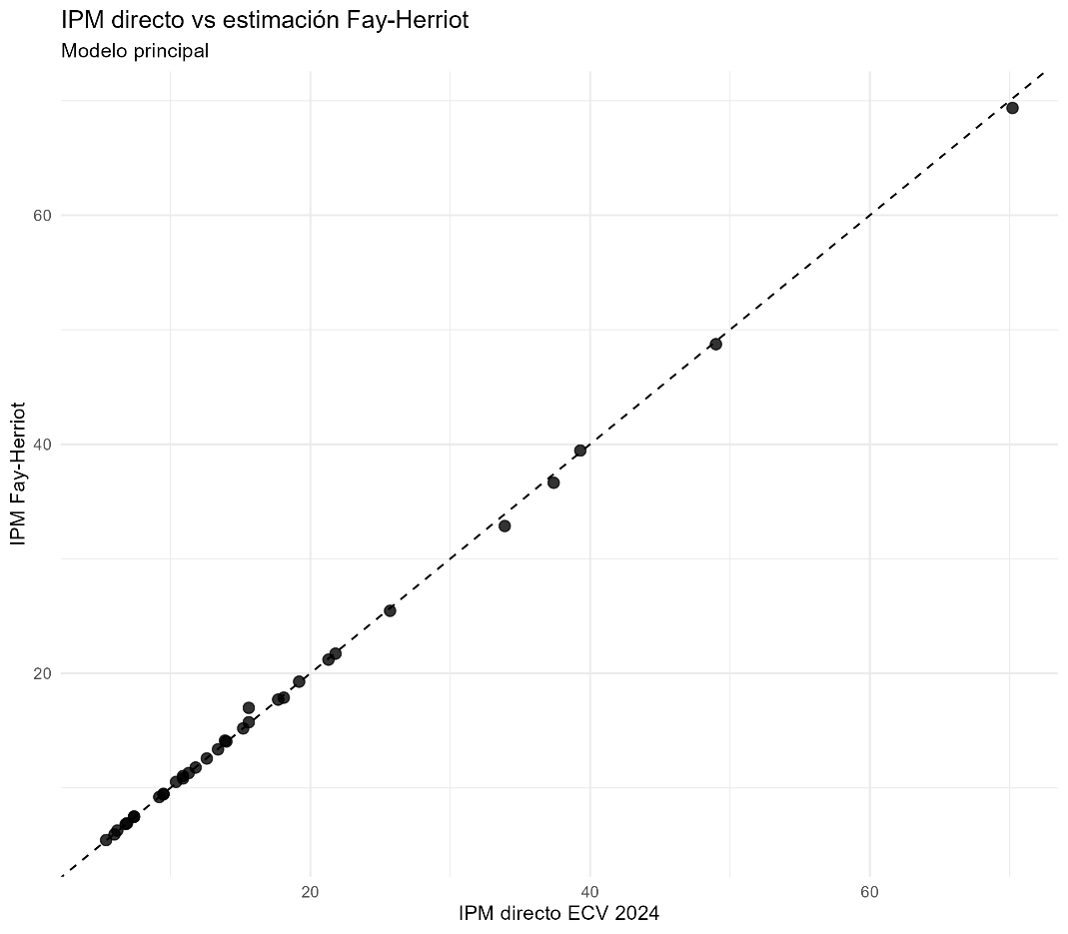
\includegraphics[width=0.65\textwidth]{fig/figures/IPM_Fay-Herriot.png}
    \caption{}
    \textbf{Fuente:} elaboración propia con base en estimaciones del script de modelamiento.
\end{figure}

La diferencia entre el modelo principal y el modelo de sensibilidad también fue reducida a nivel departamental. La diferencia promedio entre ambas estimaciones fue de -0,016 puntos, con un mínimo de -0,520 y un máximo de 0,463. Esto sugiere que, a escala departamental, las estimaciones son relativamente estables frente al cambio en la especificación de la variable de mortalidad infantil.

\begin{figure}[H]
    \centering
    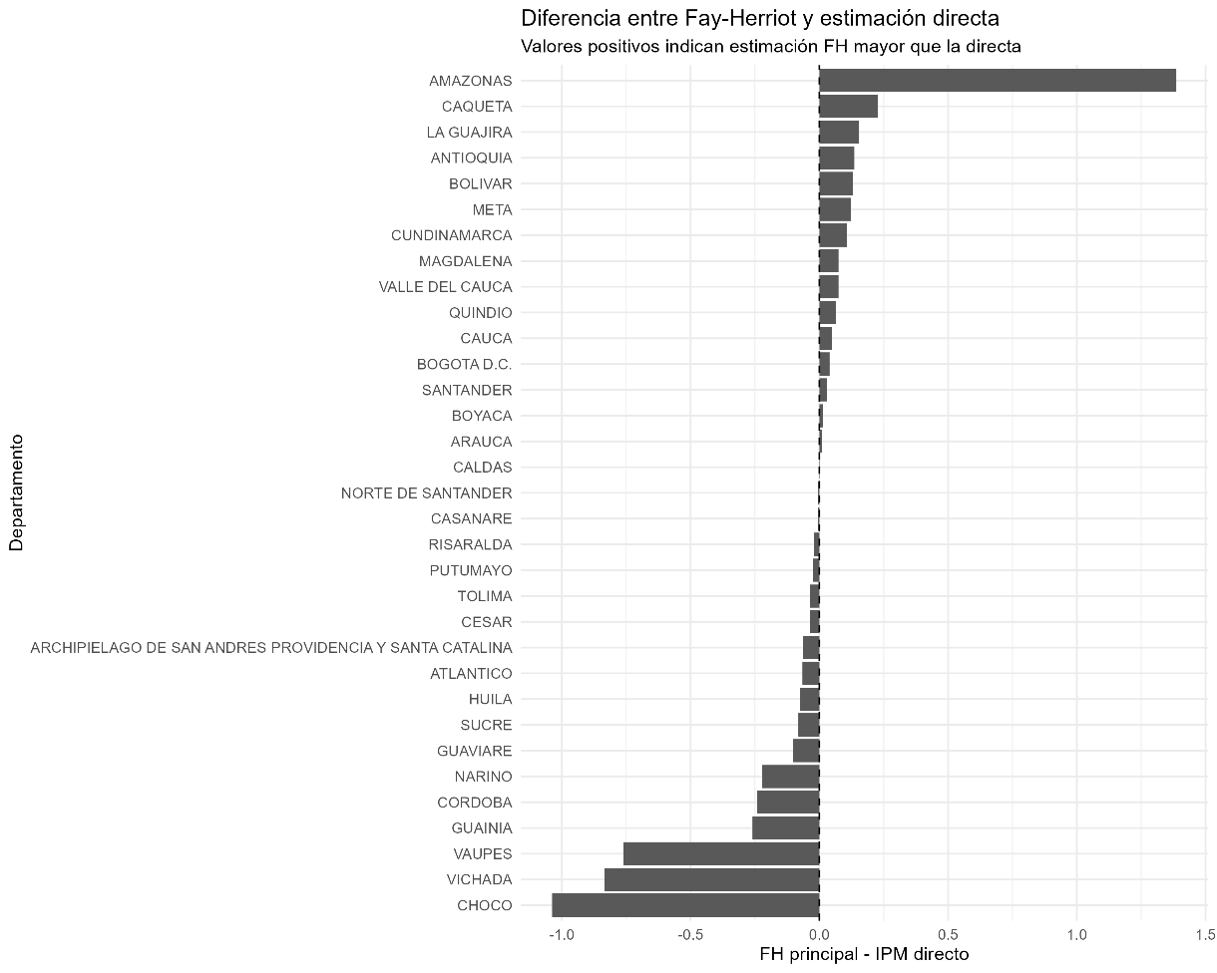
\includegraphics[width=0.65\textwidth]{fig/figures/Diferencia_Fay_Herriot-Directa.png}
    \caption{}
    \textbf{Fuente:} elaboración propia con base en estimaciones del script de modelamiento.
\end{figure}

Adicionalmente, se estimó el error cuadrático medio (MSE) del modelo Fay–Herriot. En el modelo principal, los valores de MSE se ubicaron aproximadamente entre 0,49 y 5,03, mientras que en el modelo de sensibilidad se ubicaron entre 0,49 y 5,10. Estos resultados permiten aproximar la incertidumbre asociada a las estimaciones suavizadas y constituyen un insumo relevante para comparar la precisión relativa entre departamentos.

El error estándar asociado al estimador se obtuvo mediante:

\begin{equation}
SE_{FH,d} = \sqrt{MSE_d}
\end{equation}

\begin{figure}[H]
    \centering
    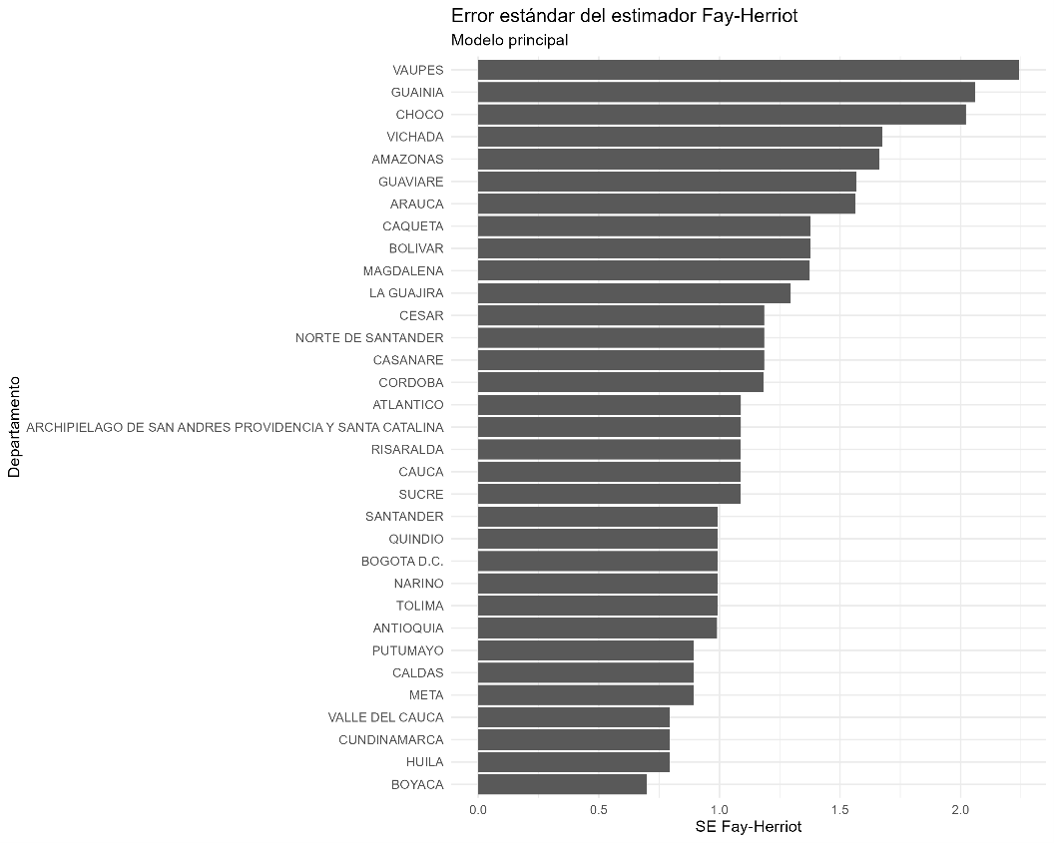
\includegraphics[width=0.65\textwidth]{fig/figures/Error_estandar_Fay-Herrot.png}
    \caption{}
    \textbf{Fuente:} elaboración propia con base en el MSE del modelo Fay–Herriot principal.
\end{figure}

\section{Predicción sintética municipal del IPM 2024}
Con base en los coeficientes estimados en los modelos Fay–Herriot, se generó una predicción sintética municipal del IPM 2024. Se aplicaron los parámetros del modelo departamental sobre la matriz de covariables municipales junto al efecto departamental estimado $\hat{u}_d$.

Las predicciones fueron acotadas entre 0 y 100 para mantener coherencia con la escala del IPM. El modelo principal se expresa entonces de manera general como:

\begin{equation}
    \begin{split}        
        IPM_{m,d} = -13,84 + 393,71(\text{repitencia}_{m,d}) - 18,48(\text{infraestructura básica}_{m,d}) \\ + 0,12(\text{mortalidad infantil}_{m,d}) + \hat{u}_d
    \end{split}
\end{equation}

Para asegurar consistencia, los resultados fueron acotados entre 0 y 100:

\begin{equation}
    IPM_{m,d}\text{ acotado} = \min[100, \max(0, IPM_{m,d})]
\end{equation}

Donde:

\begin{itemize}
    \item $IPM_{m,d}$: IPM predicho para el municipio $m$ perteneciente al departamento $d$.
    \item $\text{repitencia}_{m,d}$: repitencia del municipio $m$ en el departamento $d$.
    \item $\text{infraestructura básica}_{m,d}$: índice de infraestructura básica del municipio $m$ en el departamento $d$.
    \item $\text{mortalidad infantil}_{m,d}$: mortalidad infantil del municipio $m$ en el departamento $d$.
    \item $\hat{u}_d$: efecto departamental estimado por el modelo Fay–Herriot.
\end{itemize}

En el modelo principal, la distribución del IPM municipal predicho acotado presentó un mínimo de 0, una mediana de 10,02, una media de 13,61 y un máximo de 100. En el modelo de sensibilidad, la mediana fue de 11,86, la media de 14,91 y el rango también estuvo entre 0 y 100.

\begin{figure}[H]
    \centering
    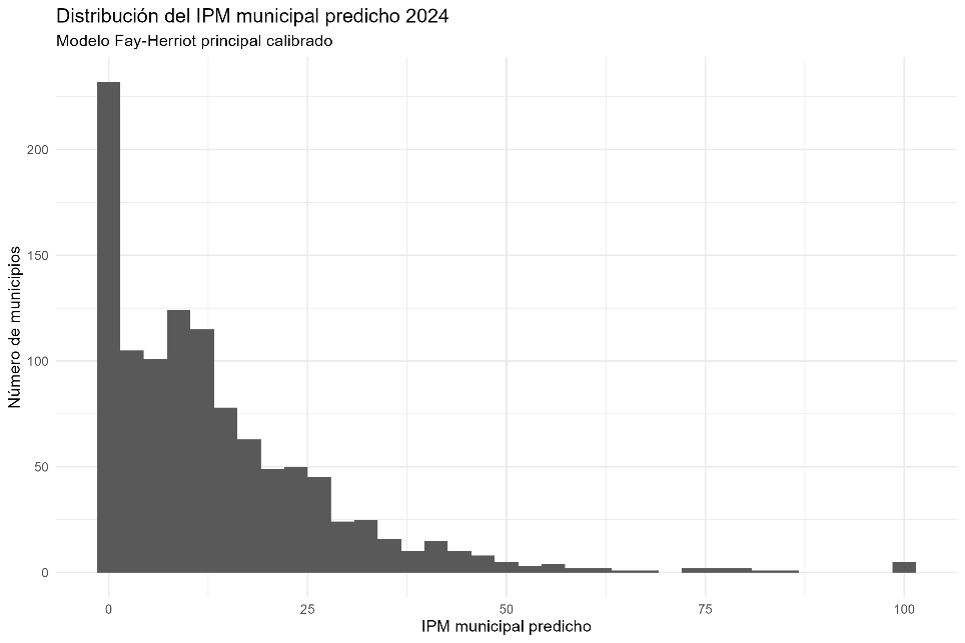
\includegraphics[width=0.65\textwidth]{fig/figures/IPM_predict_2024.png}
    \caption{}
    \textbf{Fuente:} elaboración propia con base en la comparación de predicciones municipales.
\end{figure}

La presencia de valores extremos antes del acotamiento refleja que el modelo extrapola con fuerza en algunos territorios, por lo que estas predicciones deben tomarse como un ejercicio preliminar. Por ejemplo, algunos municipios presentaron predicciones fijas superiores a 100 antes del ajuste de escala.

La diferencia entre las predicciones municipales del modelo principal y el modelo de sensibilidad se calculó como:

\begin{equation}
    \begin{split}
        \text{Diferencia}_{m,d} = \text{IPM principal}_{m,d} - \text{IPM sensibilidad}_{m,d}
    \end{split}
\end{equation}

La comparación entre el modelo principal y el modelo de sensibilidad mostró diferencias importantes en algunos municipios. Aunque la diferencia promedio entre modelos fue baja, se observaron casos con discrepancias elevadas, lo cual evidencia sensibilidad de las predicciones municipales frente a la especificación funcional de la variable de salud. Esto refuerza la necesidad de incorporar ajustes adicionales, tales como control de valores extremos, evaluación de covariables influyentes y procedimientos de calibración o benchmarking departamental.

\begin{figure}[H]
    \centering
    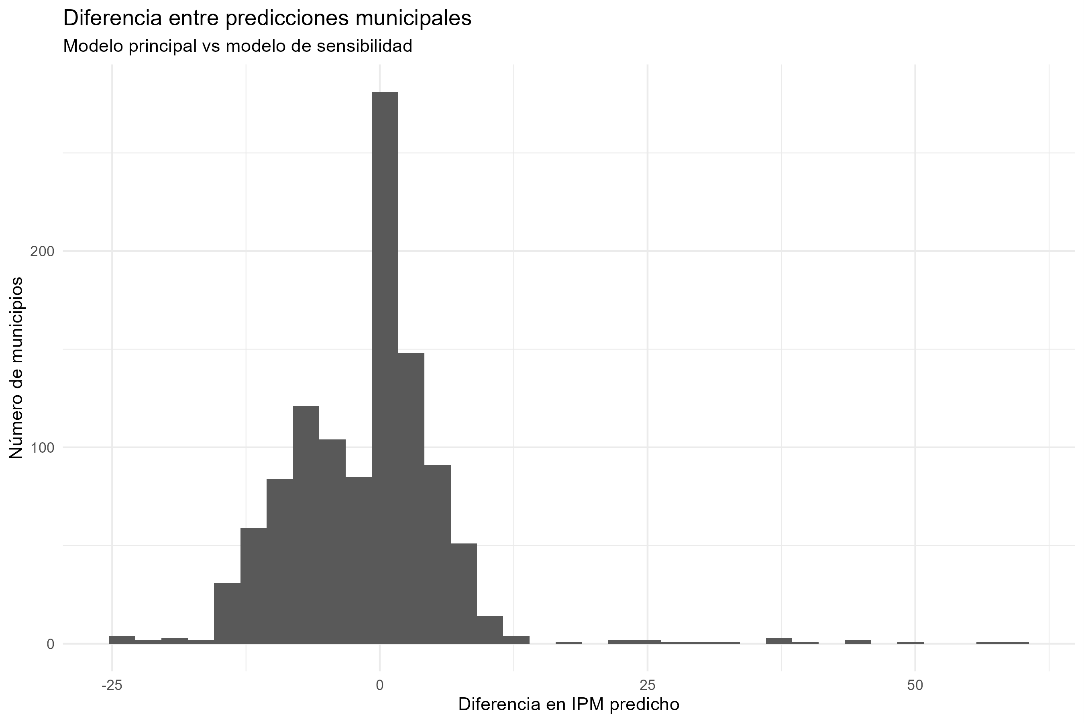
\includegraphics[width=0.65\textwidth]{fig/figures/Dif_predict_mpales.png}
    \caption{}
    \textbf{Fuente:} elaboración propia con base en la comparación de predicciones municipales.
\end{figure}

\section{Validación agregada departamental}
Como ejercicio de validación interna, se calculó el promedio del IPM municipal predicho dentro de cada departamento y se comparó con el IPM directo departamental de la ECV 2024. Esta validación no reemplaza una validación externa, pero permite evaluar si las predicciones municipales conservan la estructura territorial agregada utilizada como ancla del modelo.

El promedio municipal predicho por departamento se calculó como:

\begin{equation}
    IPM\text{ promedio}_d = \frac{1}{N_d} \sum IPM_{m,d}
\end{equation}

Los resultados arrojaron una alta correlación de 0,924 frente al IPM directo departamental de la ECV, con un RMSE de 5,36 y un MAE de 2,60. Estos valores sugieren que el modelo conserva de manera general el patrón departamental del IPM, aunque con diferencias relevantes en algunos territorios.

Las métricas formales se estructuran de la siguiente manera:

\begin{align}
    RMSE &= \sqrt{\frac{1}{D} \sum (IPM\text{ directo}_d - IPM\text{ promedio}_d)^2} 
\end{align}
\begin{align}
    MAE &= \frac{1}{D} \sum |IPM\text{ directo}_d - IPM\text{ promedio}_d|
\end{align}

Los resultados pueden apreciarse a continuación:

\begin{figure}[H]
    \centering
    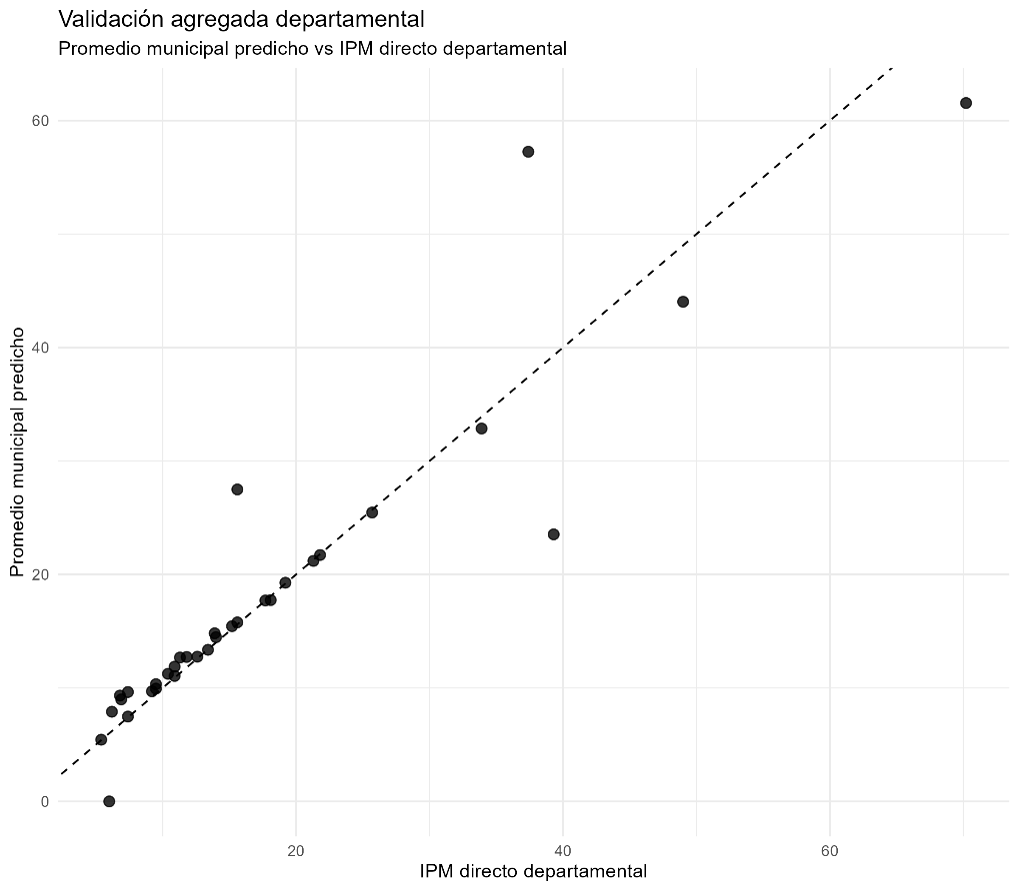
\includegraphics[width=0.65\textwidth]{fig/figures/Validacion_dptal.png}
    \caption{}
    \textbf{Fuente:} elaboración propia con base en predicciones municipales agregadas por departamento.
\end{figure}

A pesar de la alta correlación, se observaron brechas importantes en departamentos específicos como La Guajira ($-15,77$ puntos de diferencia), Amazonas ($+11,89$), Vaupés ($+19,85$), Vichada ($-8,65$) y San Andrés ($-6,00$), sugiriendo la necesidad de un proceso posterior de calibración o \textit{benchmarking}: las diferencias muestran que, aunque el modelo reproduce adecuadamente la estructura general, requiere una etapa posterior de ajuste para mejorar la coherencia entre el nivel municipal y el nivel departamental.

\section{Diagnóstico espacial preliminar}
Se aplicó la prueba global de Moran sobre los residuos de la especificación principal utilizando el criterio de contigüidad tipo reina:

\begin{equation}
    \begin{split}    
        I = \frac{D}{S_0} \frac{\sum_i \sum_j w_{ij}(e_i - \bar{e})(e_j - \bar{e})}{\sum_i (e_i - \bar{e})^2}
    \end{split}
\end{equation}

Donde:
\begin{itemize}
    \item $I$: estadístico global de Moran.
    \item $D$: número de departamentos.
    \item $w_{ij}$: peso espacial entre los departamentos $i$ y $j$.
    \item $e_i$ y $e_j$: residuos del modelo en los departamentos $i$ y $j$.
    \item $\bar{e}$: promedio de los residuos.
    \item $S_0$: suma total de los pesos espaciales.
\end{itemize}

El estadístico obtenido fue de $-0,097$ con un valor-p de $0,732$. Al ser el valor-p mayor a 0,05, no hay evidencia de auto correlación espacial positiva en los residuos departamentales, indicando que las covariables capturan satisfactoriamente la estructura territorial general. Sin embargo, debido a advertencias por discontinuidades geográficas o islas, se aconseja interpretar con cautela y explorar otras matrices de pesos.

No obstante, el procedimiento generó advertencias relacionadas con la existencia de departamentos sin vecinos y la presencia de subgrafos en la matriz de vecindad. Esto puede estar asociado a territorios insulares o a discontinuidades geográficas en la estructura departamental. Por esta razón, el diagnóstico espacial debe interpretarse con cautela y se recomienda explorar matrices de pesos alternativas, como vecinos más cercanos o criterios de distancia.

El modelo Fay–Herriot principal es consistente y conceptualmente interpretable: la repitencia se asocia al rezago educativo; la infraestructura básica refleja condiciones de vivienda y servicios; y la mortalidad infantil actúa como proxy de vulnerabilidad sanitaria. Los siguientes pasos analíticos se enfocarán en refinar la calibración municipal, corregir las predicciones en municipios atípicos y ensayar formulaciones espaciales más robustas.

%%--------------------------------------------------
%\section{Limpieza, filtrado y reglas explícitas}
   

%%--------------------------------------------------
%\section{Identificación de datos faltantes}
   


%%--------------------------------------------------
%\section{Ventanas temporales y partición de los datos en conjuntos de entrenamiento y prueba}

    
        
%%--------------------------------------------------
%\section{Construcción de variables predictoras}

    
%%--------------------------------------------------
%\section{Construcción de la variable respuesta}

    
    
%%--------------------------------------------------
%\section{Análisis exploratorio}
    
    
%%--------------------------------------------------
%\section{Preprocesamiento}


%%--------------------------------------------------
%\section{Construcción de matrices de diseño del modelo \emph{pogit}}

 
    
%%--------------------------------------------------
%\section{Reducción de dimensionalidad y segmentación ex-
%ploratoria} 


%--------------------------------------------------
%\section{Resultados de la estimación del modelo \emph{pogit}}

    
    
        
    